We crawled Twitter data using Twitter Streaming API for two years spanning 2013 and 2014 years. This type of crawling provides us with a very sparse set of data, roughly $1\%$ of all tweets \footnote{\hyperref[]{http://allthingsd.com/20101110/twitter-firehose-too-intense-take-a-sip-from-the-garden-hose-or-sample-the-spritzer|}}. The total number of tweets collected is $829,026,458$. In the context of Twitter, we consider a list of $5$ features for each tweet. Each tweet has a $From$, the person who tweeted it, and a $Time$ which is the date information of the tweet. It can also contain 
\begin{itemize}
\item $Hashtag(s)$, keywords specified using \# sign
\item $Mention(s)$, another Twitter username being mentioned using @ sign
\item $Term(s)$, uni-grams which we extract from the 140 characters of the tweet. These uni-grams are later cleaned to remove $Term$s with no meaning (total number of $Term$s before cleaning was $20,234,729$)
\end{itemize}
Table \ref{table:featureStatistics} provides more detail statistics about each feature. For each feature, we reported the count of the feature in our dataset, in addition to maximum, average, median counts of each feature across the tweets. Lower part of the table provides these counts across user dimension meaning that for example a hashtag has been used in average by $10.08$ users. Last part of the table shows the statistics for the hashtag usage of our users e.g., users have used $2$ hashtags in average.

%%%%%%%%%%%%%%%%%%%%%%%%%%%%%%%%%%%%%%%%%%%%%%%%%%%%%%%%%%%%%%%%%%%%%%%%%%%
\begin{figure*}[tbph!]
\centering
\begin{tabular}{ccc}
\begin{tabular}{ccc}
\subfloat[Fig:][Human Caused Disaster]{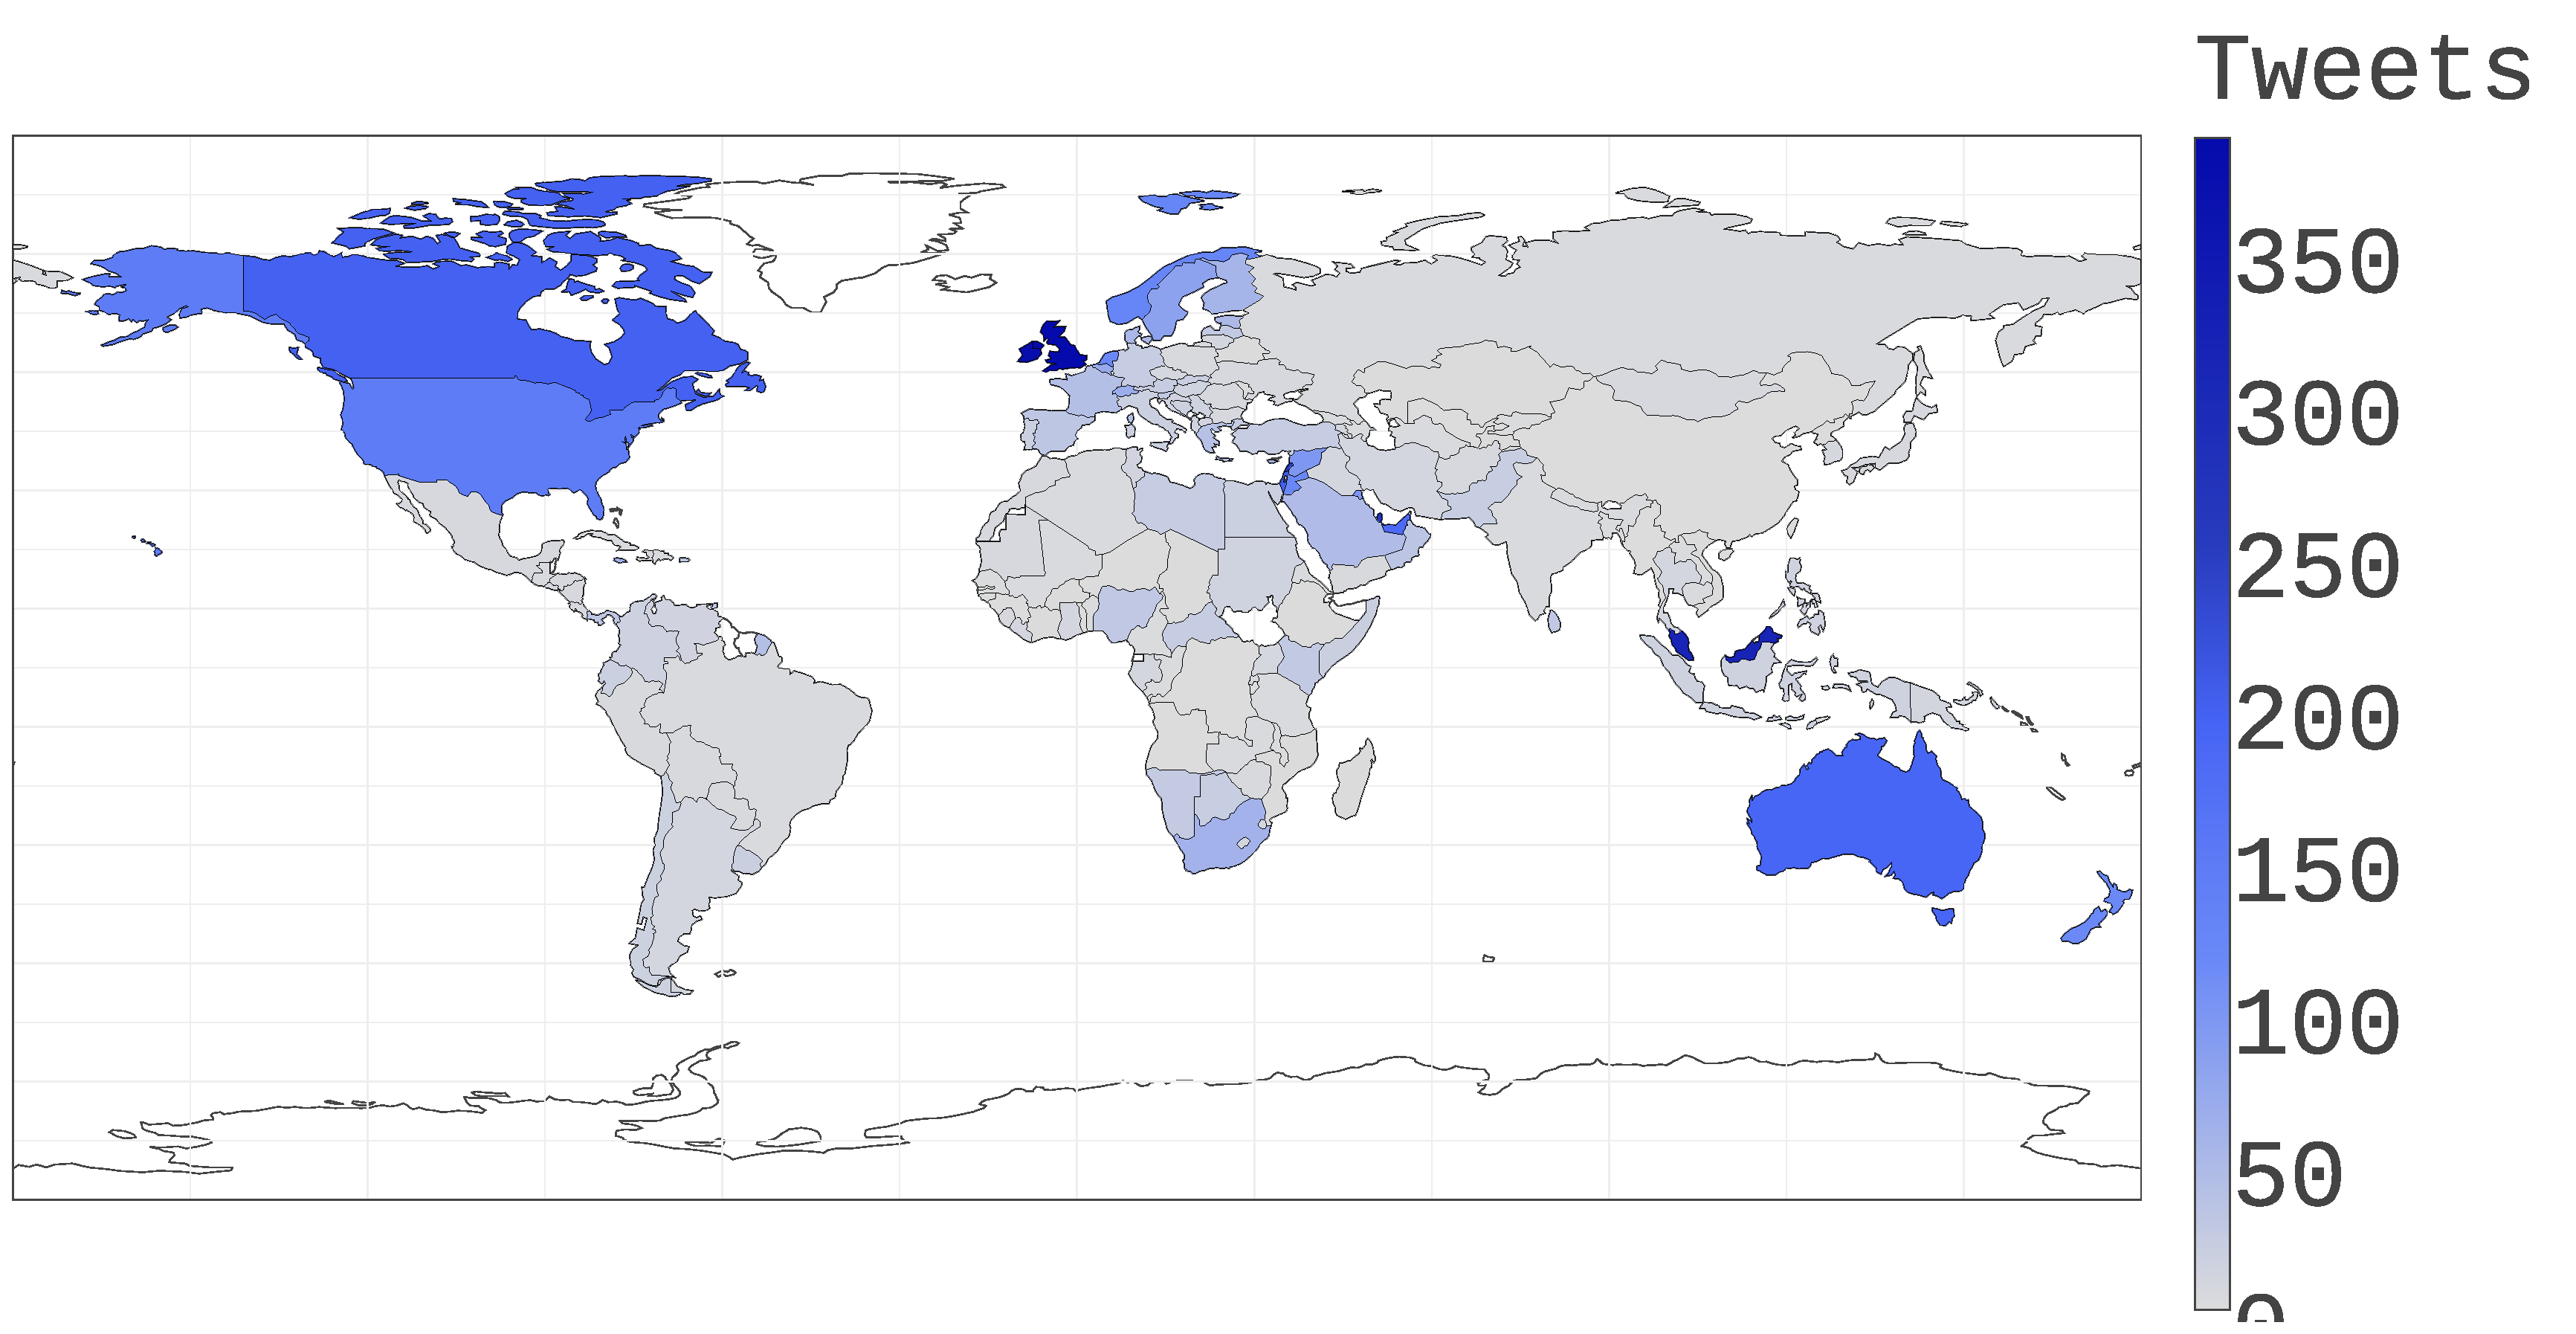
\includegraphics[width=5.3cm]{images/location/world/socialsensor-world-humancauseddisaster_location.eps}}
\subfloat[Fig:][Iran Deal]{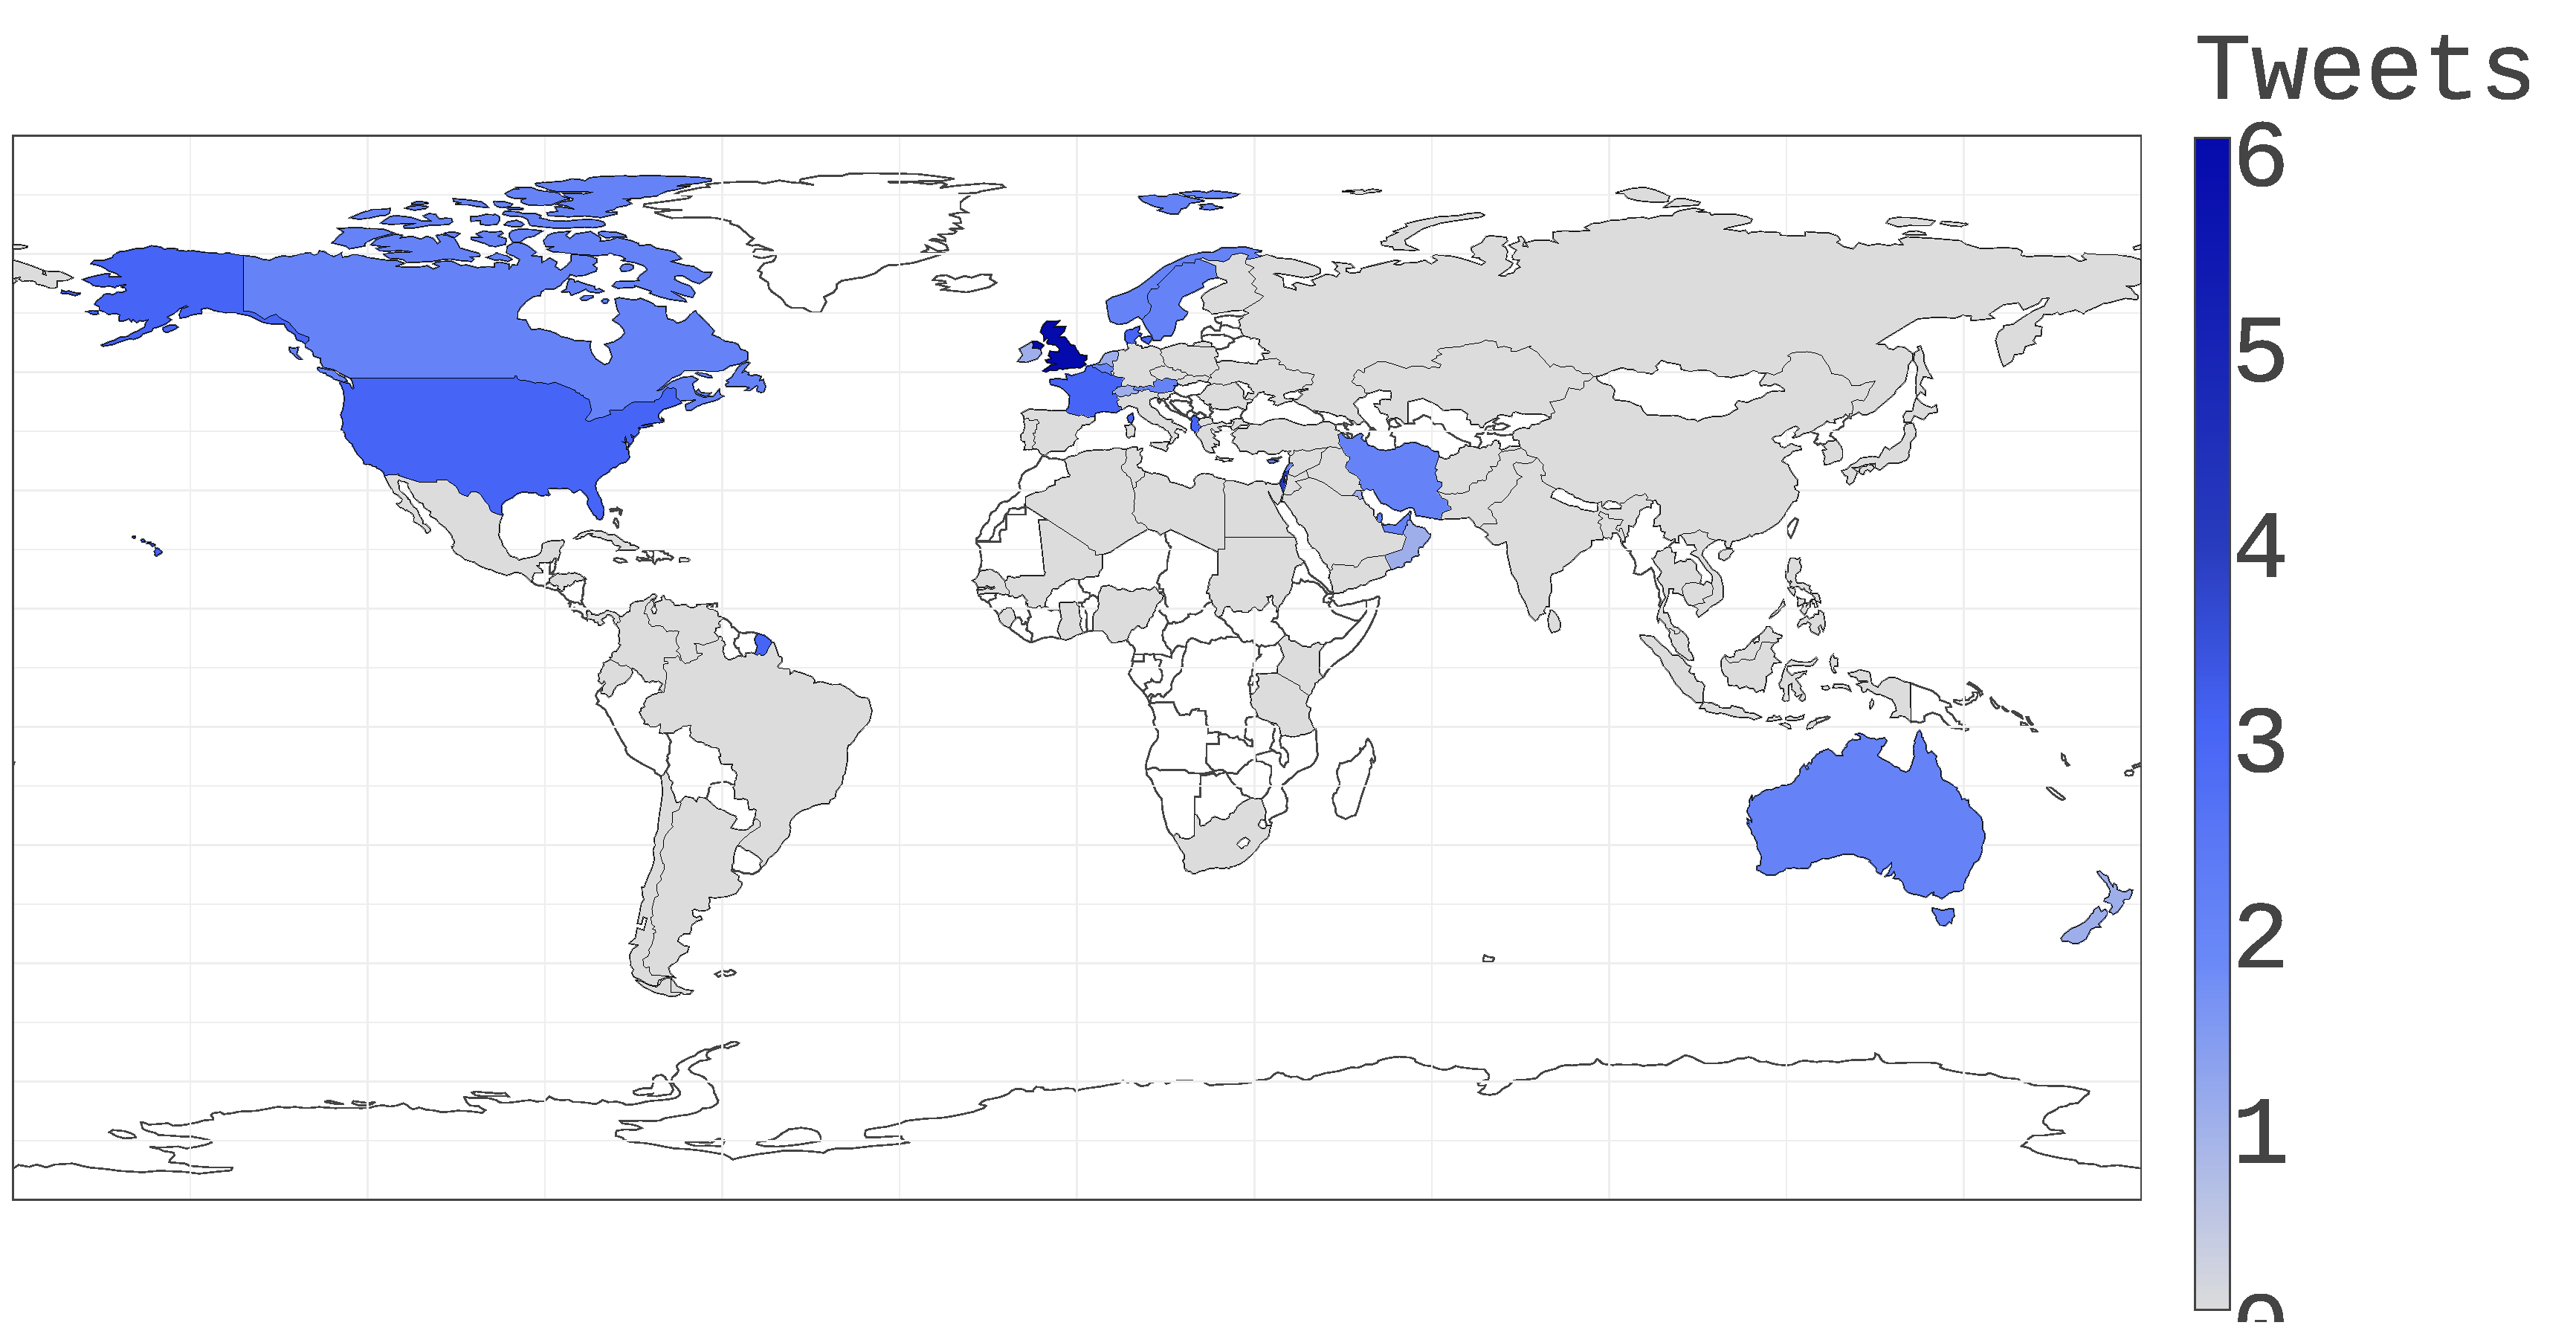
\includegraphics[width=5.3cm]{images/location/world/socialsensor-world-irannucleardeal_location.eps}}
\subfloat[Fig:][Soccer]{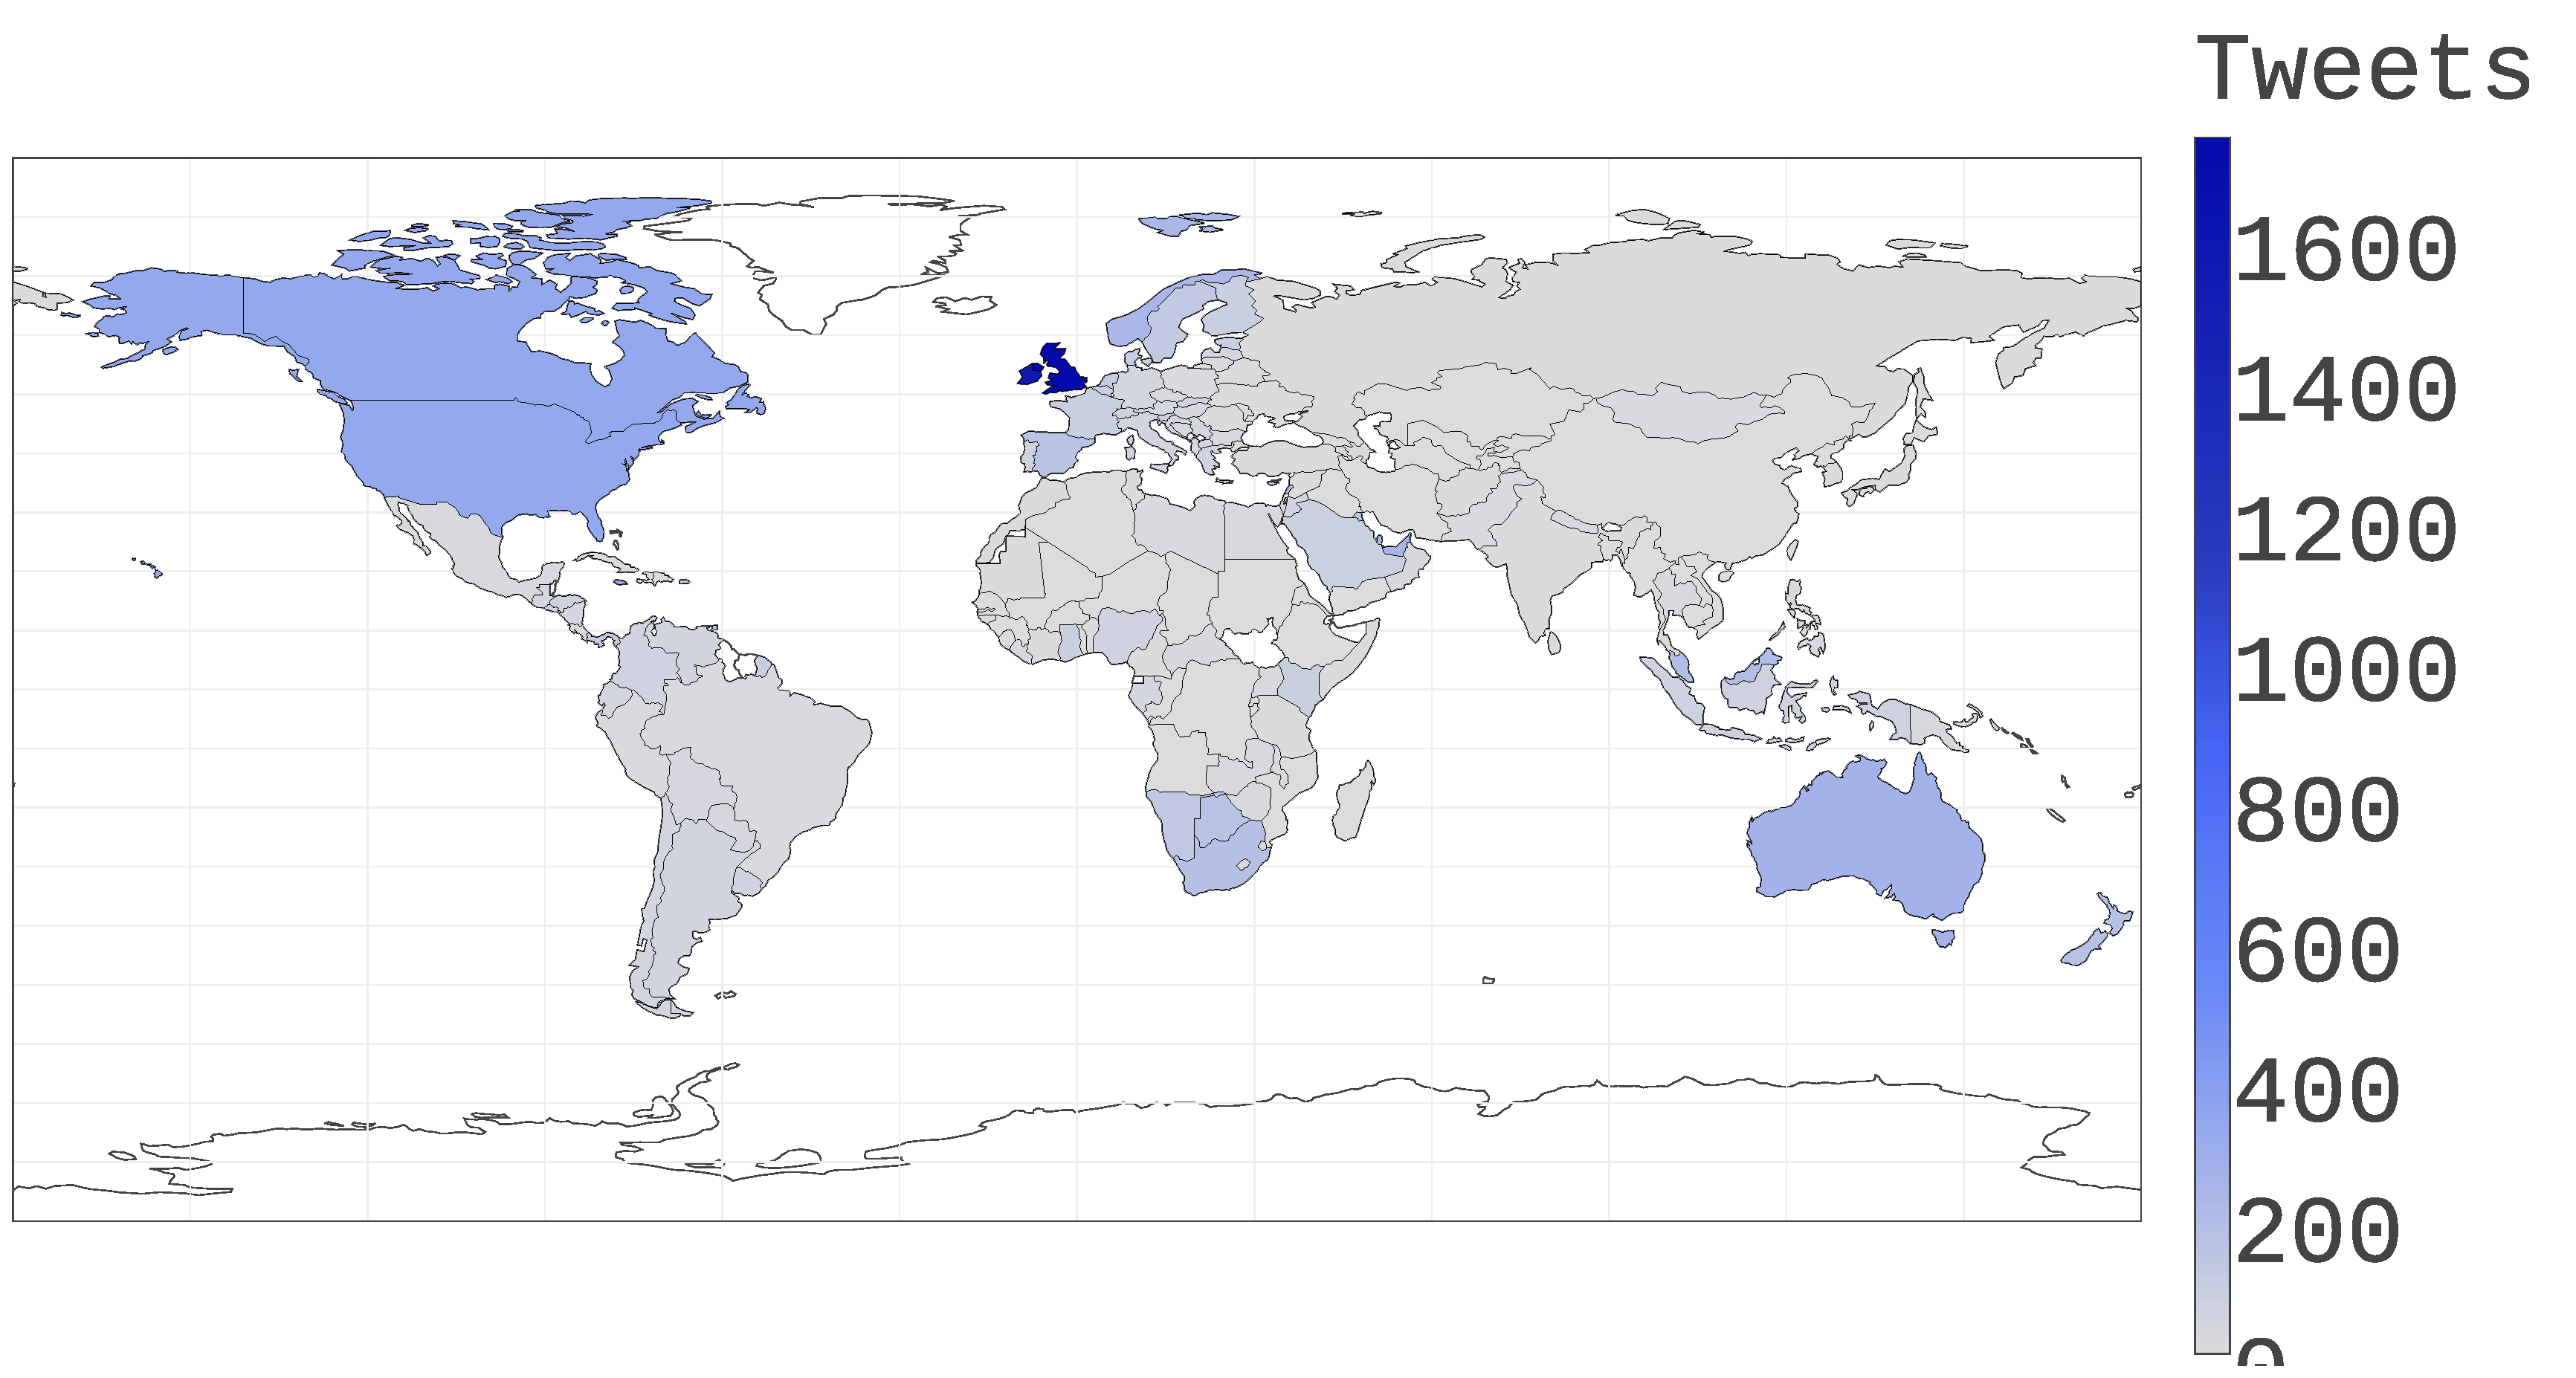
\includegraphics[width=5.3cm]{images/location/world/socialsensor-world-soccer_location.eps}} \\
%\vspace{-10mm}
\subfloat[Fig:][Health Epidemics]{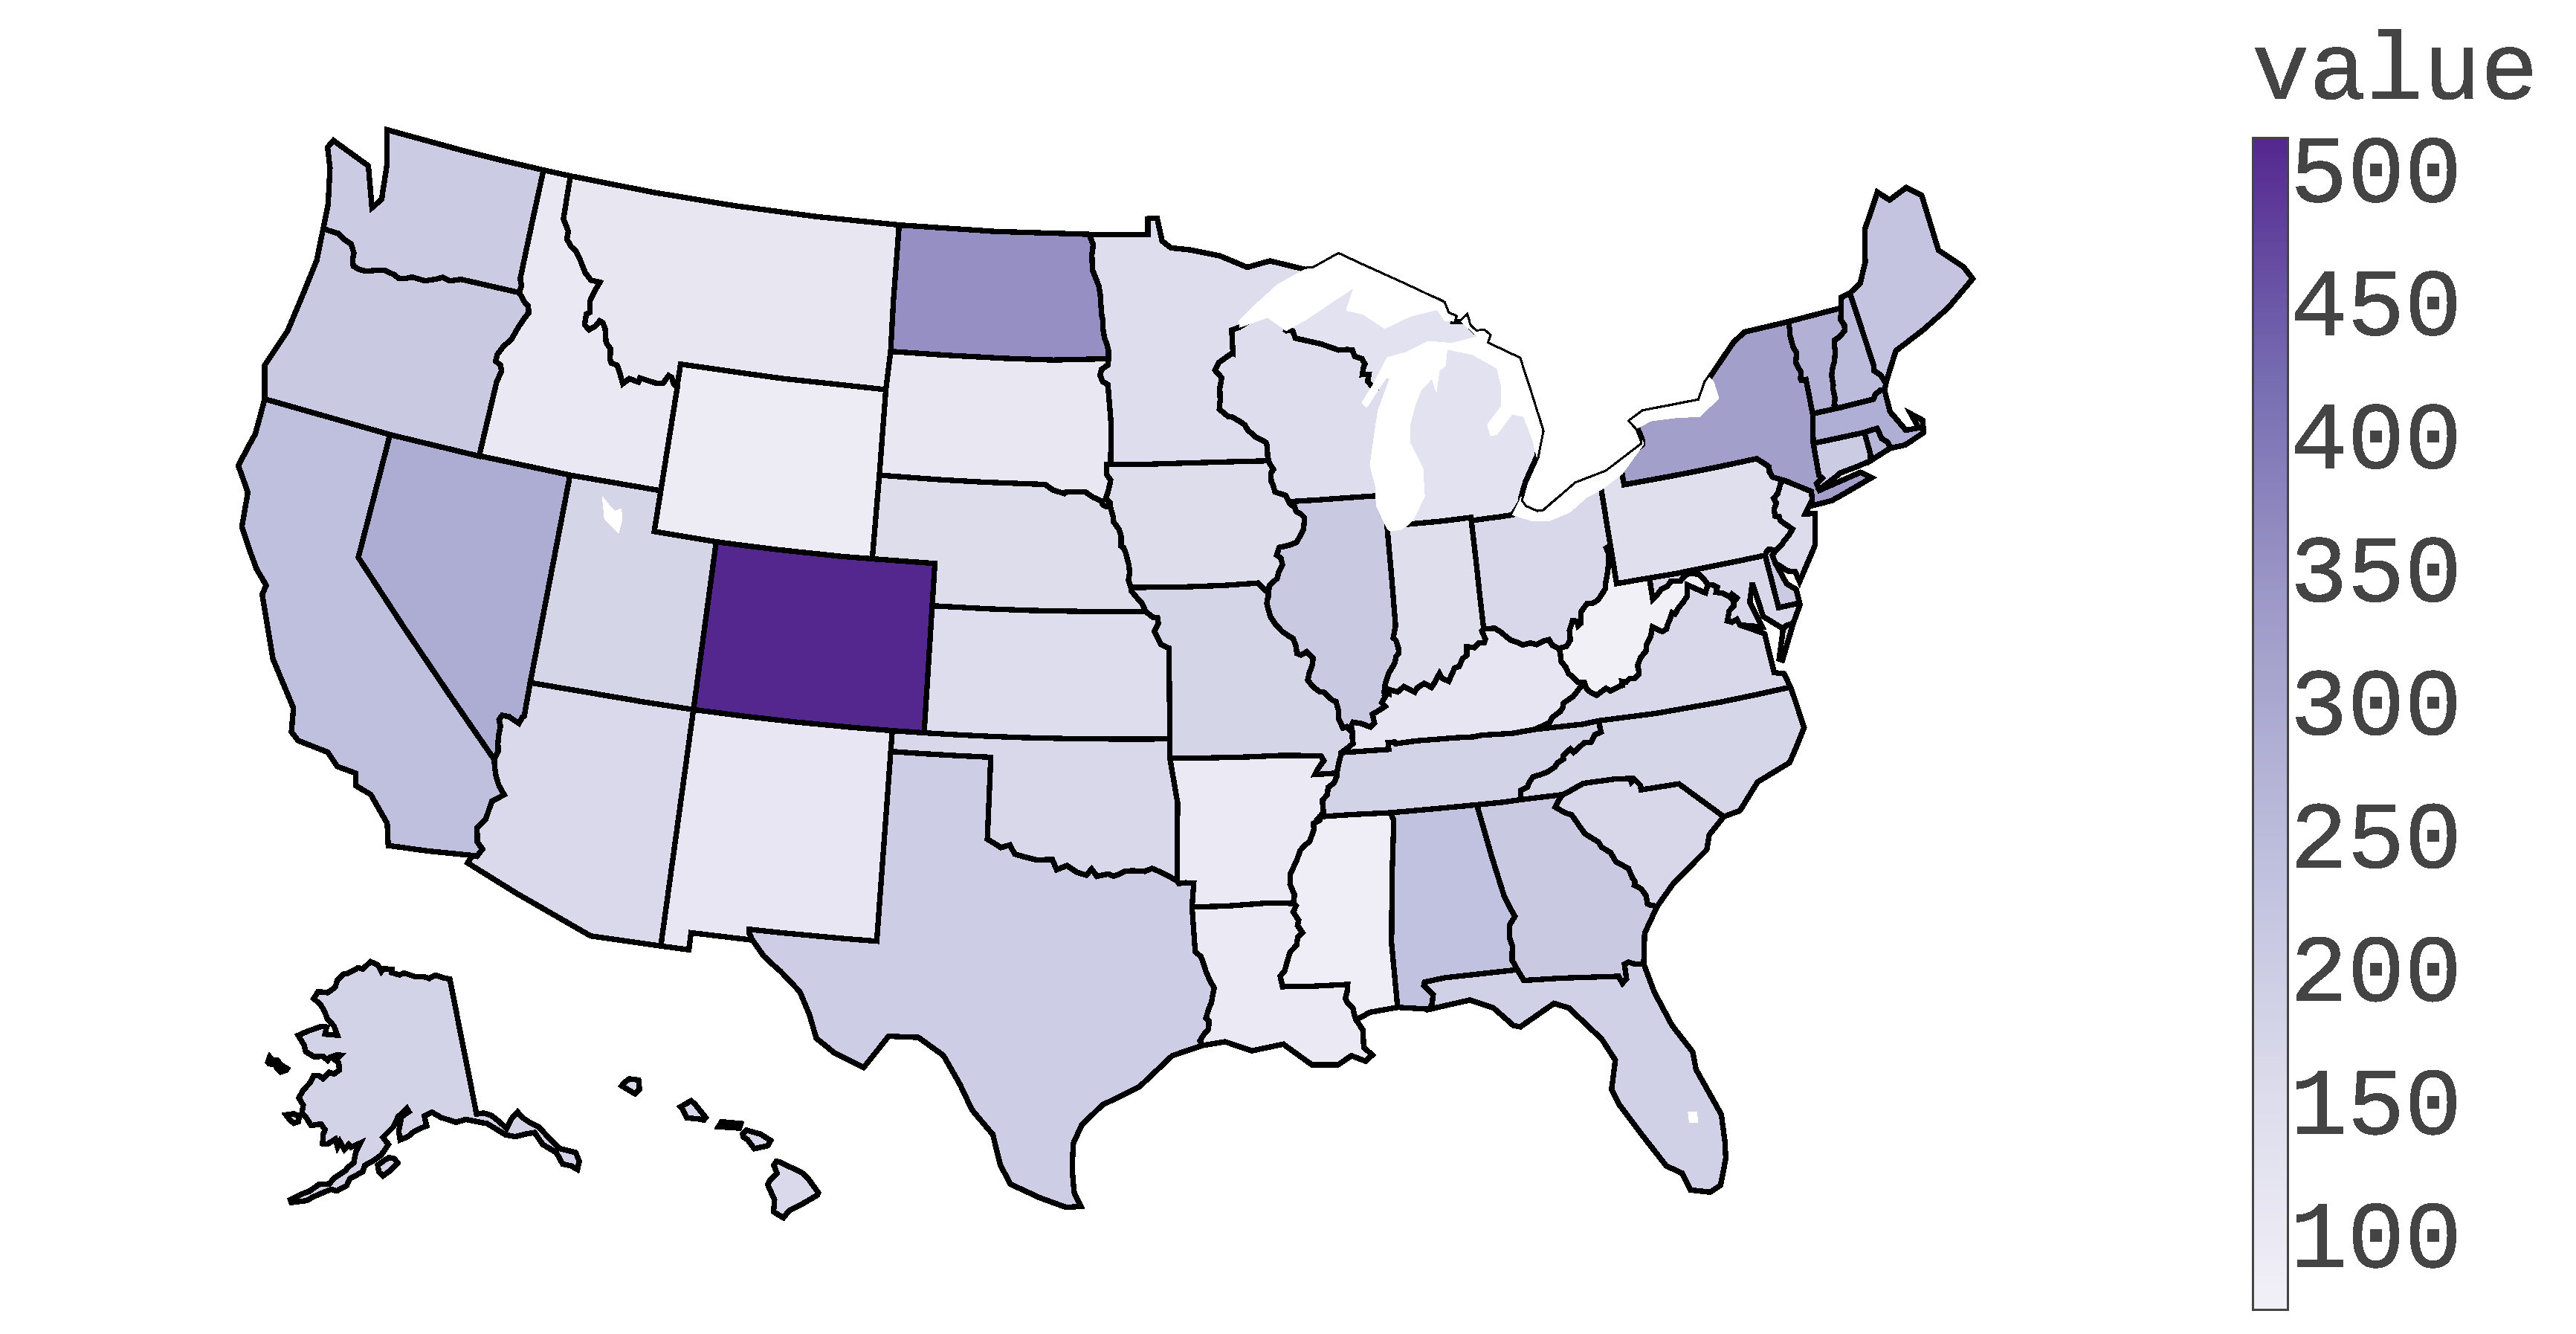
\includegraphics[width=5.3cm]{images/location/states/SocialSensor-us-states-health_epidemics_location.eps}}
\subfloat[Fig:][Social Issues]{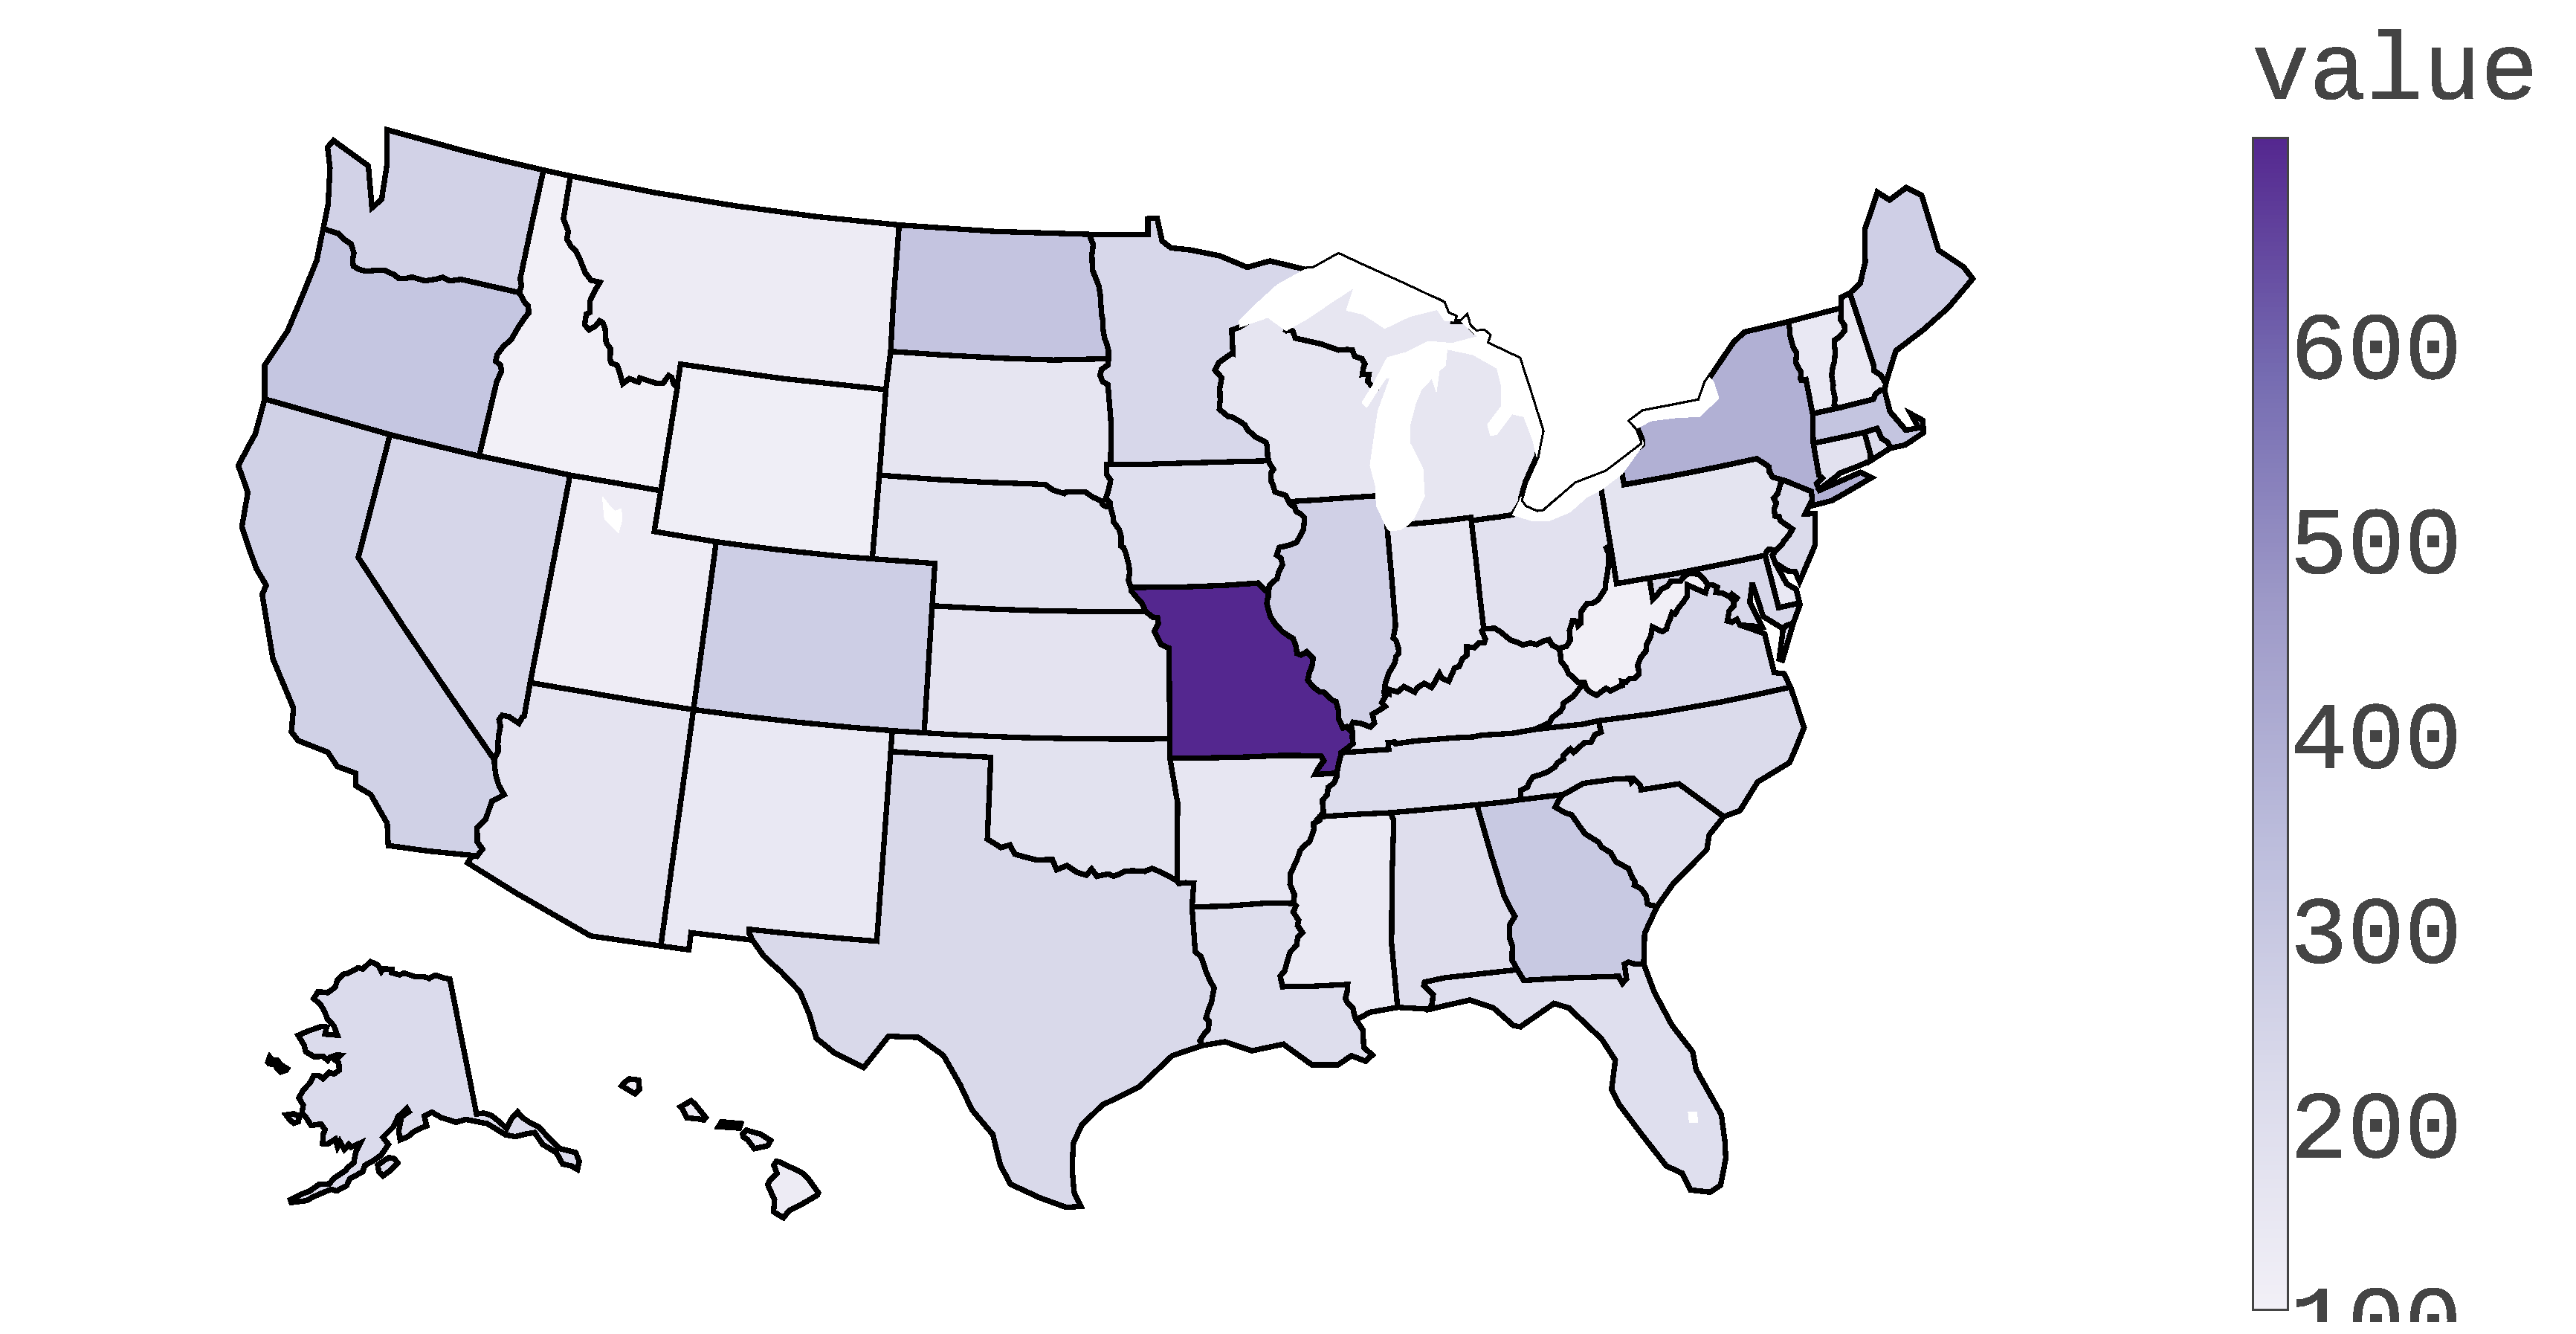
\includegraphics[width=5.3cm]{images/location/states/SocialSensor-us-states-socialissues_location.eps}}
\subfloat[Fig:][Space]{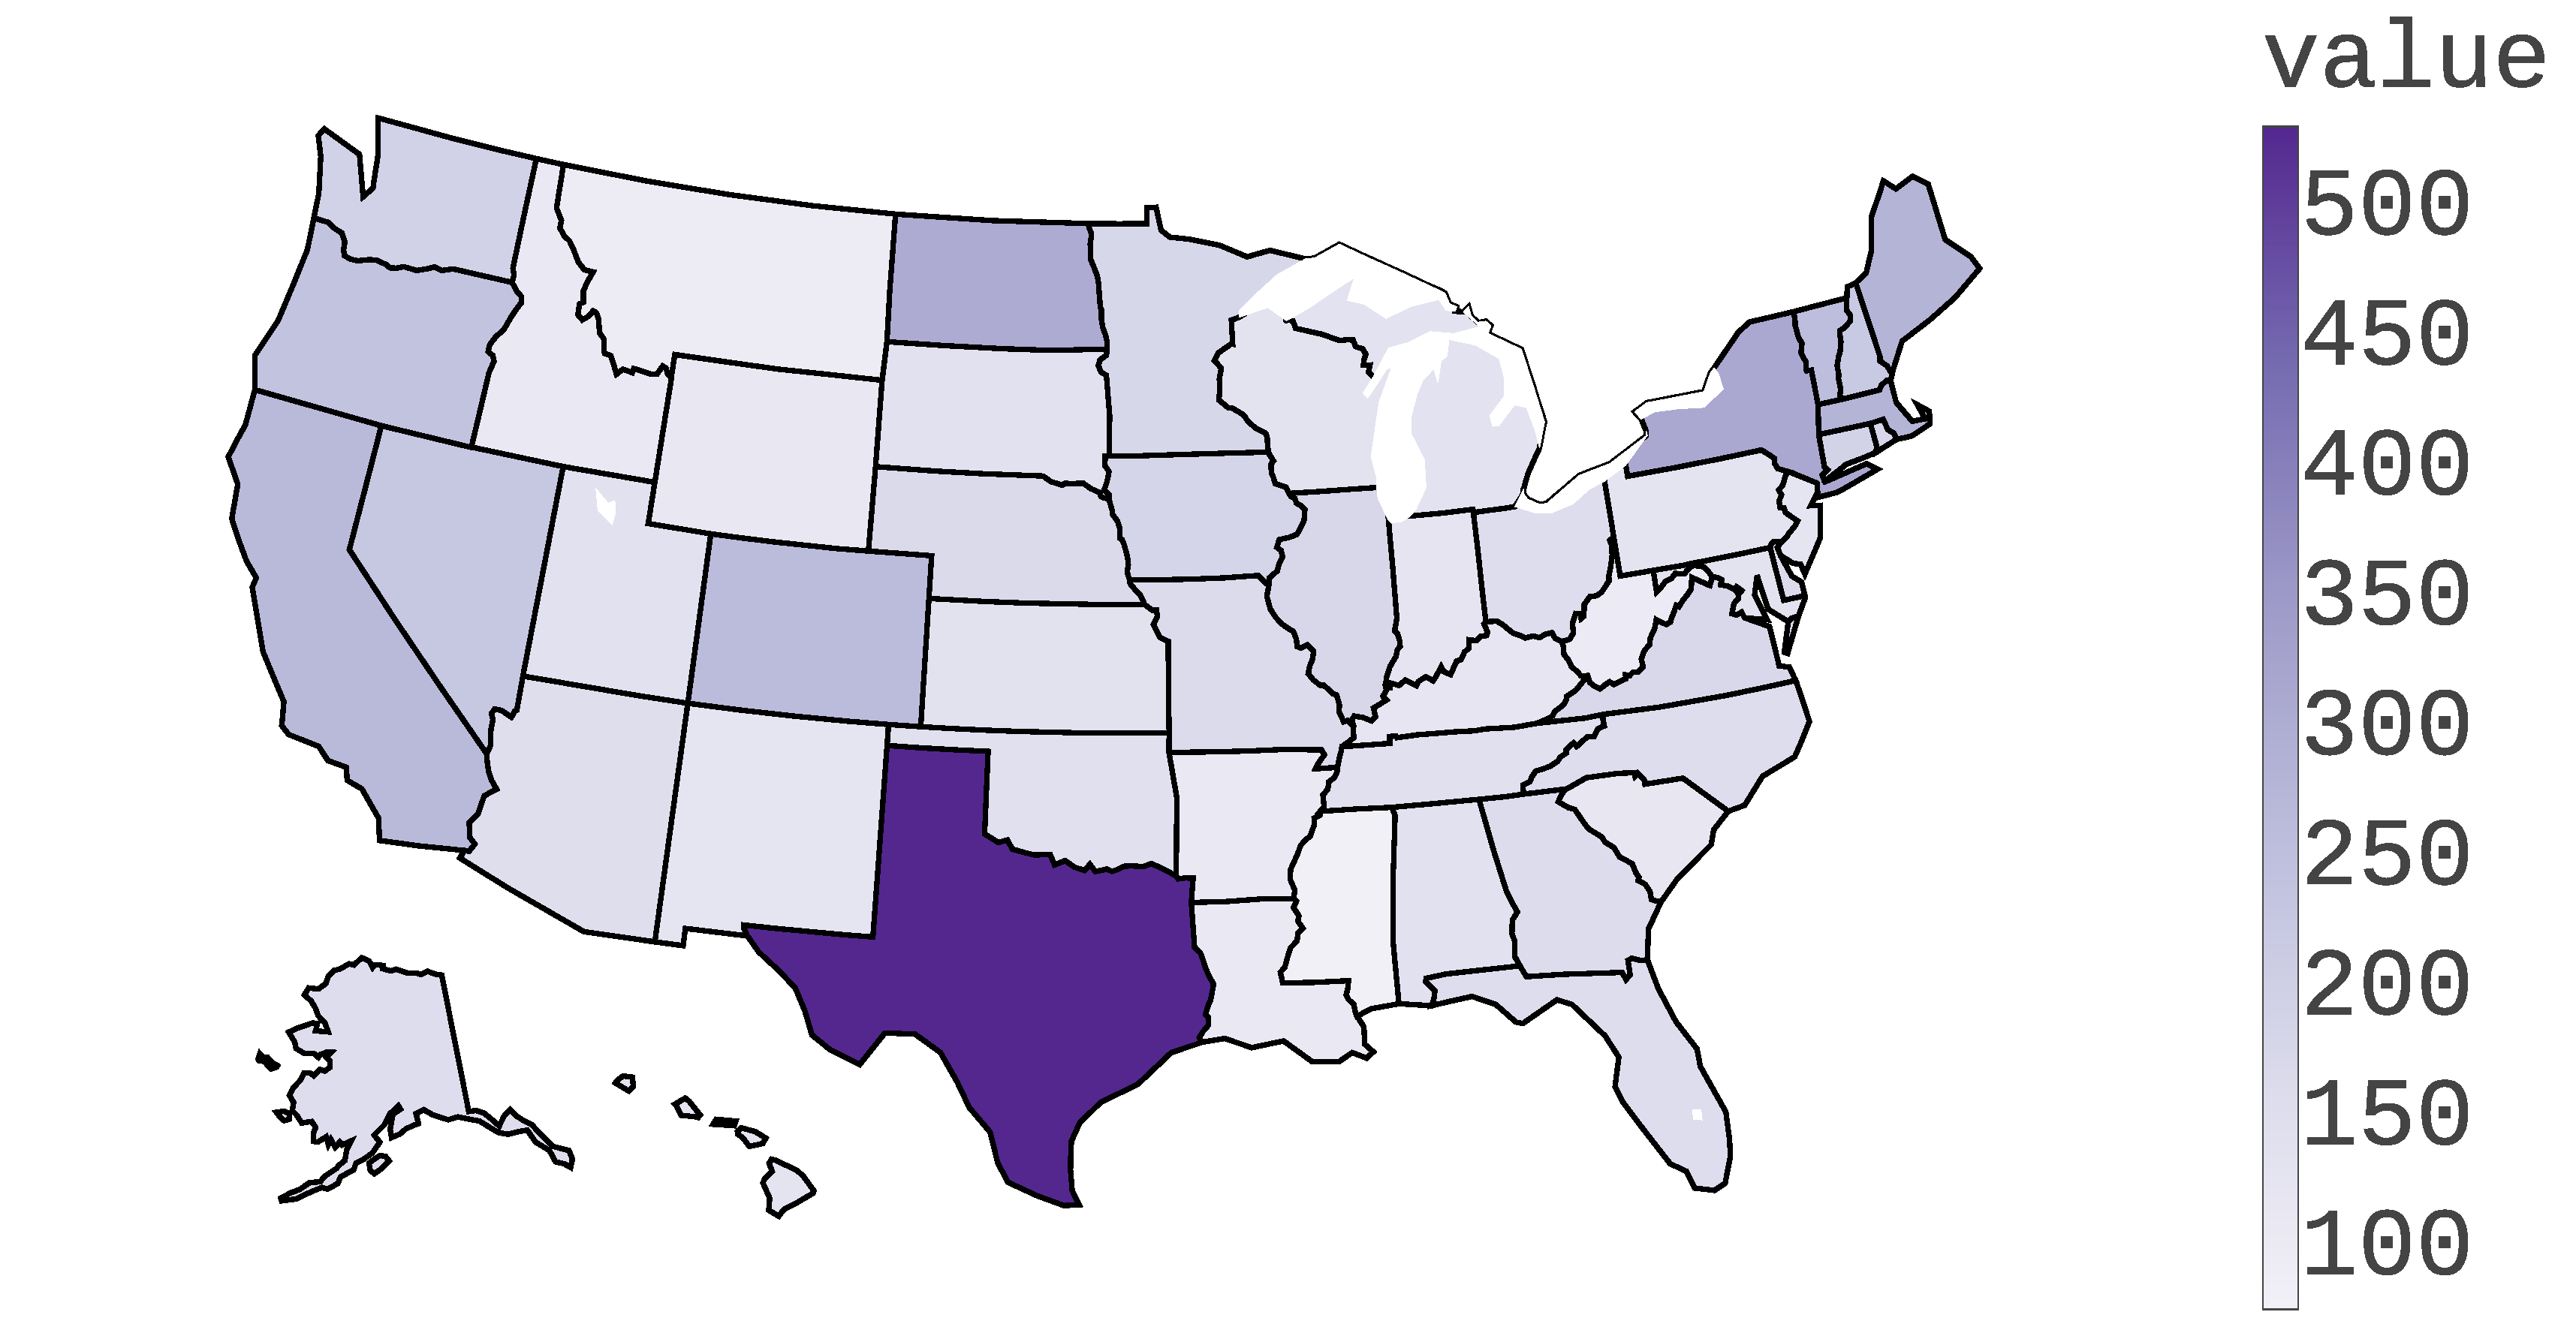
\includegraphics[width=5.3cm]{images/location/states/SocialSensor-us-states-space_location}} \\
\end{tabular}
\end{tabular}
\vspace{-2mm}
\caption {Choropleths of top: International map and bottom: U.S. map }
\label{fig:choropleths}
\end{figure*}
%%%%%%%%%%%%%%%%%%%%%%%%%%%%%%%%%%%%%%%%%%%%%%%%%%%%%%%%%%%%%%%%%%%%%%%%%%%


%%%%%%%%%%%%%%%%%%%%%%%%%%%%%%%%%%%%%%%%%%%%%%%%%%%%%%%%%%%%%%%%%%
\begin{table}[t!]
\centering
{\renewcommand{\arraystretch}{1.2}
\resizebox{0.5\textwidth}{!}{%
\begin{tabular}{|l|c|c|c|c|r|}
\hline
                                       & \multicolumn{4}{c|}{\textbf{Tweets}}                                                          & \textbf{}                           \\ \hline
\multicolumn{1}{|c|}{\textbf{Feature}} & \textbf{Max}          & \textbf{Avg}          & \textbf{Median}       & \textbf{Max entity}   & \multicolumn{1}{c|}{\textbf{Count}} \\ \hline
\textbf{From}                          & 10,196                & 8.67                  & 2                     & running\_status       & 95,547,198                          \\ \hline
\textbf{Hashtag}                       & 1,653,159             & 13.91                 & 1                     & \#retweet             & 11,183,410                          \\ \hline
\textbf{Mention}                       &                       &                       &                       &                       & 411,341,569                         \\ \hline
\textbf{Location}                      &                       &                       &                       &                       & 58,601                              \\ \hline
\textbf{Term}                          & 2024529               & 7,450.58              & 323                   & the                & 20,234,729                          \\ \hline
\textbf{}                              & \multicolumn{4}{c|}{\textbf{Users}}                                                           &                                     \\ \hline
\textbf{Hashtag}                       & 592,363               & 10.08                 & 1                     & \#retweet             &                                     \\ \hline
\textbf{Mention}                       & 26,293                & 5.44                  & 1                     & dimensionist          &                                     \\ \hline
\textbf{Location}                      & 739,120               & 641.5                 & 2                     & london                &                                     \\ \hline
\textbf{Term}                          & 1,799,385             & 6,616.65              & 305                   & the                &                                     \\ \hline
\textbf{}                              & \multicolumn{4}{c|}{\textbf{Hashtags}}                                                        &                                     \\ \hline
\textbf{From}                          & 18,167                & 1.62                     & 0                     & daily\_astrodata      &                                     \\ \hline
\end{tabular}
}}
\caption{Feature Statistics}
\label{table:featureStatistics}
\end{table}
%%%%%%%%%%%%%%%%%%%%%%%%%%%%%%%%%%%%%%%%%%%%%%%%%%%%%%%%%%%%%%%%%%

Figure \ref{fig:tweetsStats} shows details of number of tweets per month and figure \ref{fig:powerlaw} shows the power law plots of tweet counts and hashtag counts for users. We chose $10$ topics for our experiments. Tweets are temporally divided over 2 years to provide train and test sets. Table \ref{table:sampleHashtags} provides samples of training hashtags and number of train hashtags, test hashtags, topical tweets for each topic. Some topics such as $HumanCausedDisaster$ and $Soccor$ are more general topics and have higher number of topical tweets while some other ones such as $IranDeal$ is more specific, thus having less number of topical tweets.

Figure \ref{fig:locations} shows distribution of tweets across different location in U.S. and international locations overall and for each topic(?).

%%%%%%%%%%%%%%%%%%%%%%%%%%%%%%%%%%%%%%%%%%%%%%%%%%%%%%%%%%%%%%%%%%
\begin{table*}[t!]
\centering
{\renewcommand{\arraystretch}{1.2}
\resizebox{\textwidth}{!}{%
\begin{tabular}{|l|l|l|l|l|l|l|l|l|l|l|}
\hline
\textbf{Topics/Top10} & \multicolumn{1}{c|}{\textbf{NaturalDisaster}} & \multicolumn{1}{c|}{\textbf{Epidemics}} & \multicolumn{1}{c|}{\textbf{IranDeal}} & \multicolumn{1}{c|}{\textbf{SocialIssues}} & \multicolumn{1}{c|}{\textbf{LBGT}} & \multicolumn{1}{c|}{\textbf{HumanCausedDisaster}} & \multicolumn{1}{c|}{\textbf{CelebrityDeath}} & \multicolumn{1}{c|}{\textbf{Space}} & \multicolumn{1}{c|}{\textbf{Tennis}} & \multicolumn{1}{c|}{\textbf{Soccer}} \\ \hline
\textbf{\#TrainHashtags} & \multicolumn{1}{c|}{31} & \multicolumn{1}{c|}{52} & \multicolumn{1}{c|}{12} & \multicolumn{1}{c|}{31} & \multicolumn{1}{c|}{29} & \multicolumn{1}{c|}{49} & \multicolumn{1}{c|}{28} & \multicolumn{1}{c|}{98} & \multicolumn{1}{c|}{58} & 126 \\ \hline
\textbf{\#TestHashtags} & \multicolumn{1}{c|}{18} & \multicolumn{1}{c|}{33} & \multicolumn{1}{c|}{5} & \multicolumn{1}{c|}{19} & \multicolumn{1}{c|}{17} & \multicolumn{1}{c|}{29} & \multicolumn{1}{c|}{16} & \multicolumn{1}{c|}{63} & \multicolumn{1}{c|}{36} & 81 \\ \hline
\textbf{\#TotalTopicalTweets} & \multicolumn{1}{c|}{42,987} & \multicolumn{1}{c|}{210,217} & \multicolumn{1}{c|}{8,762} & \multicolumn{1}{c|}{230,058} & \multicolumn{1}{c|}{282,527} & \multicolumn{1}{c|}{408,304} & \multicolumn{1}{c|}{163,890} & \multicolumn{1}{c|}{239,719} & \multicolumn{1}{c|}{55,053} & 860,389 \\ \hline
\multirow{5}{*}{\textbf{Sample Train Hashtags}} & \#earthquake & \#ebola & \#irandeal & \#policebrutality & \#loveislove & \#gazaunderattack & \#robinwilliams & \#asteroids & \#usopenchampion & \#worldcup \\ \cline{2-11} 
 & \#storm & \#virus & \#iranfreedom & \#michaelbrown & \#gaypride & \#childrenofsyria & \#ripmandela & \#astronauts & \#novakdjokovic & \#lovesoccer \\ \cline{2-11} 
 & \#tsunami & \#vaccine & \#irantalk & \#justice4all & \#uniteblue & \#iraqwar & \#ripjoanrivers & \#satellite & \#wimbledon & \#fifa \\ \cline{2-11} 
 & \#abfloods & \#chickenpox & \#rouhani & \#freetheweed & \#homo & \#bombthreat & \#mandela & \#spacecraft & \#womenstennis & \#realmadrid \\ \cline{2-11} 
 & \#hurricanekatrina & \#theplague & \#nuclearpower & \#newnjgunlaw & \#gaymarriage & \#isis & \#paulwalker & \#telescope & \#tennisnews & \#beckham \\ \hline
\end{tabular}
}
}
\caption{Test/Train Hashtag samples and statistics}
\label{table:sampleHashtags}
\end{table*}
%%%%%%%%%%%%%%%%%%%%%%%%%%%%%%%%%%%%%%%%%%%%%%%%%%%%%%%%%%%%%%%%%%
